\subsubsection{Quartet encoding}
\label{sec:quartet_encoding}
\begin{figure}[t!]
    \centering
    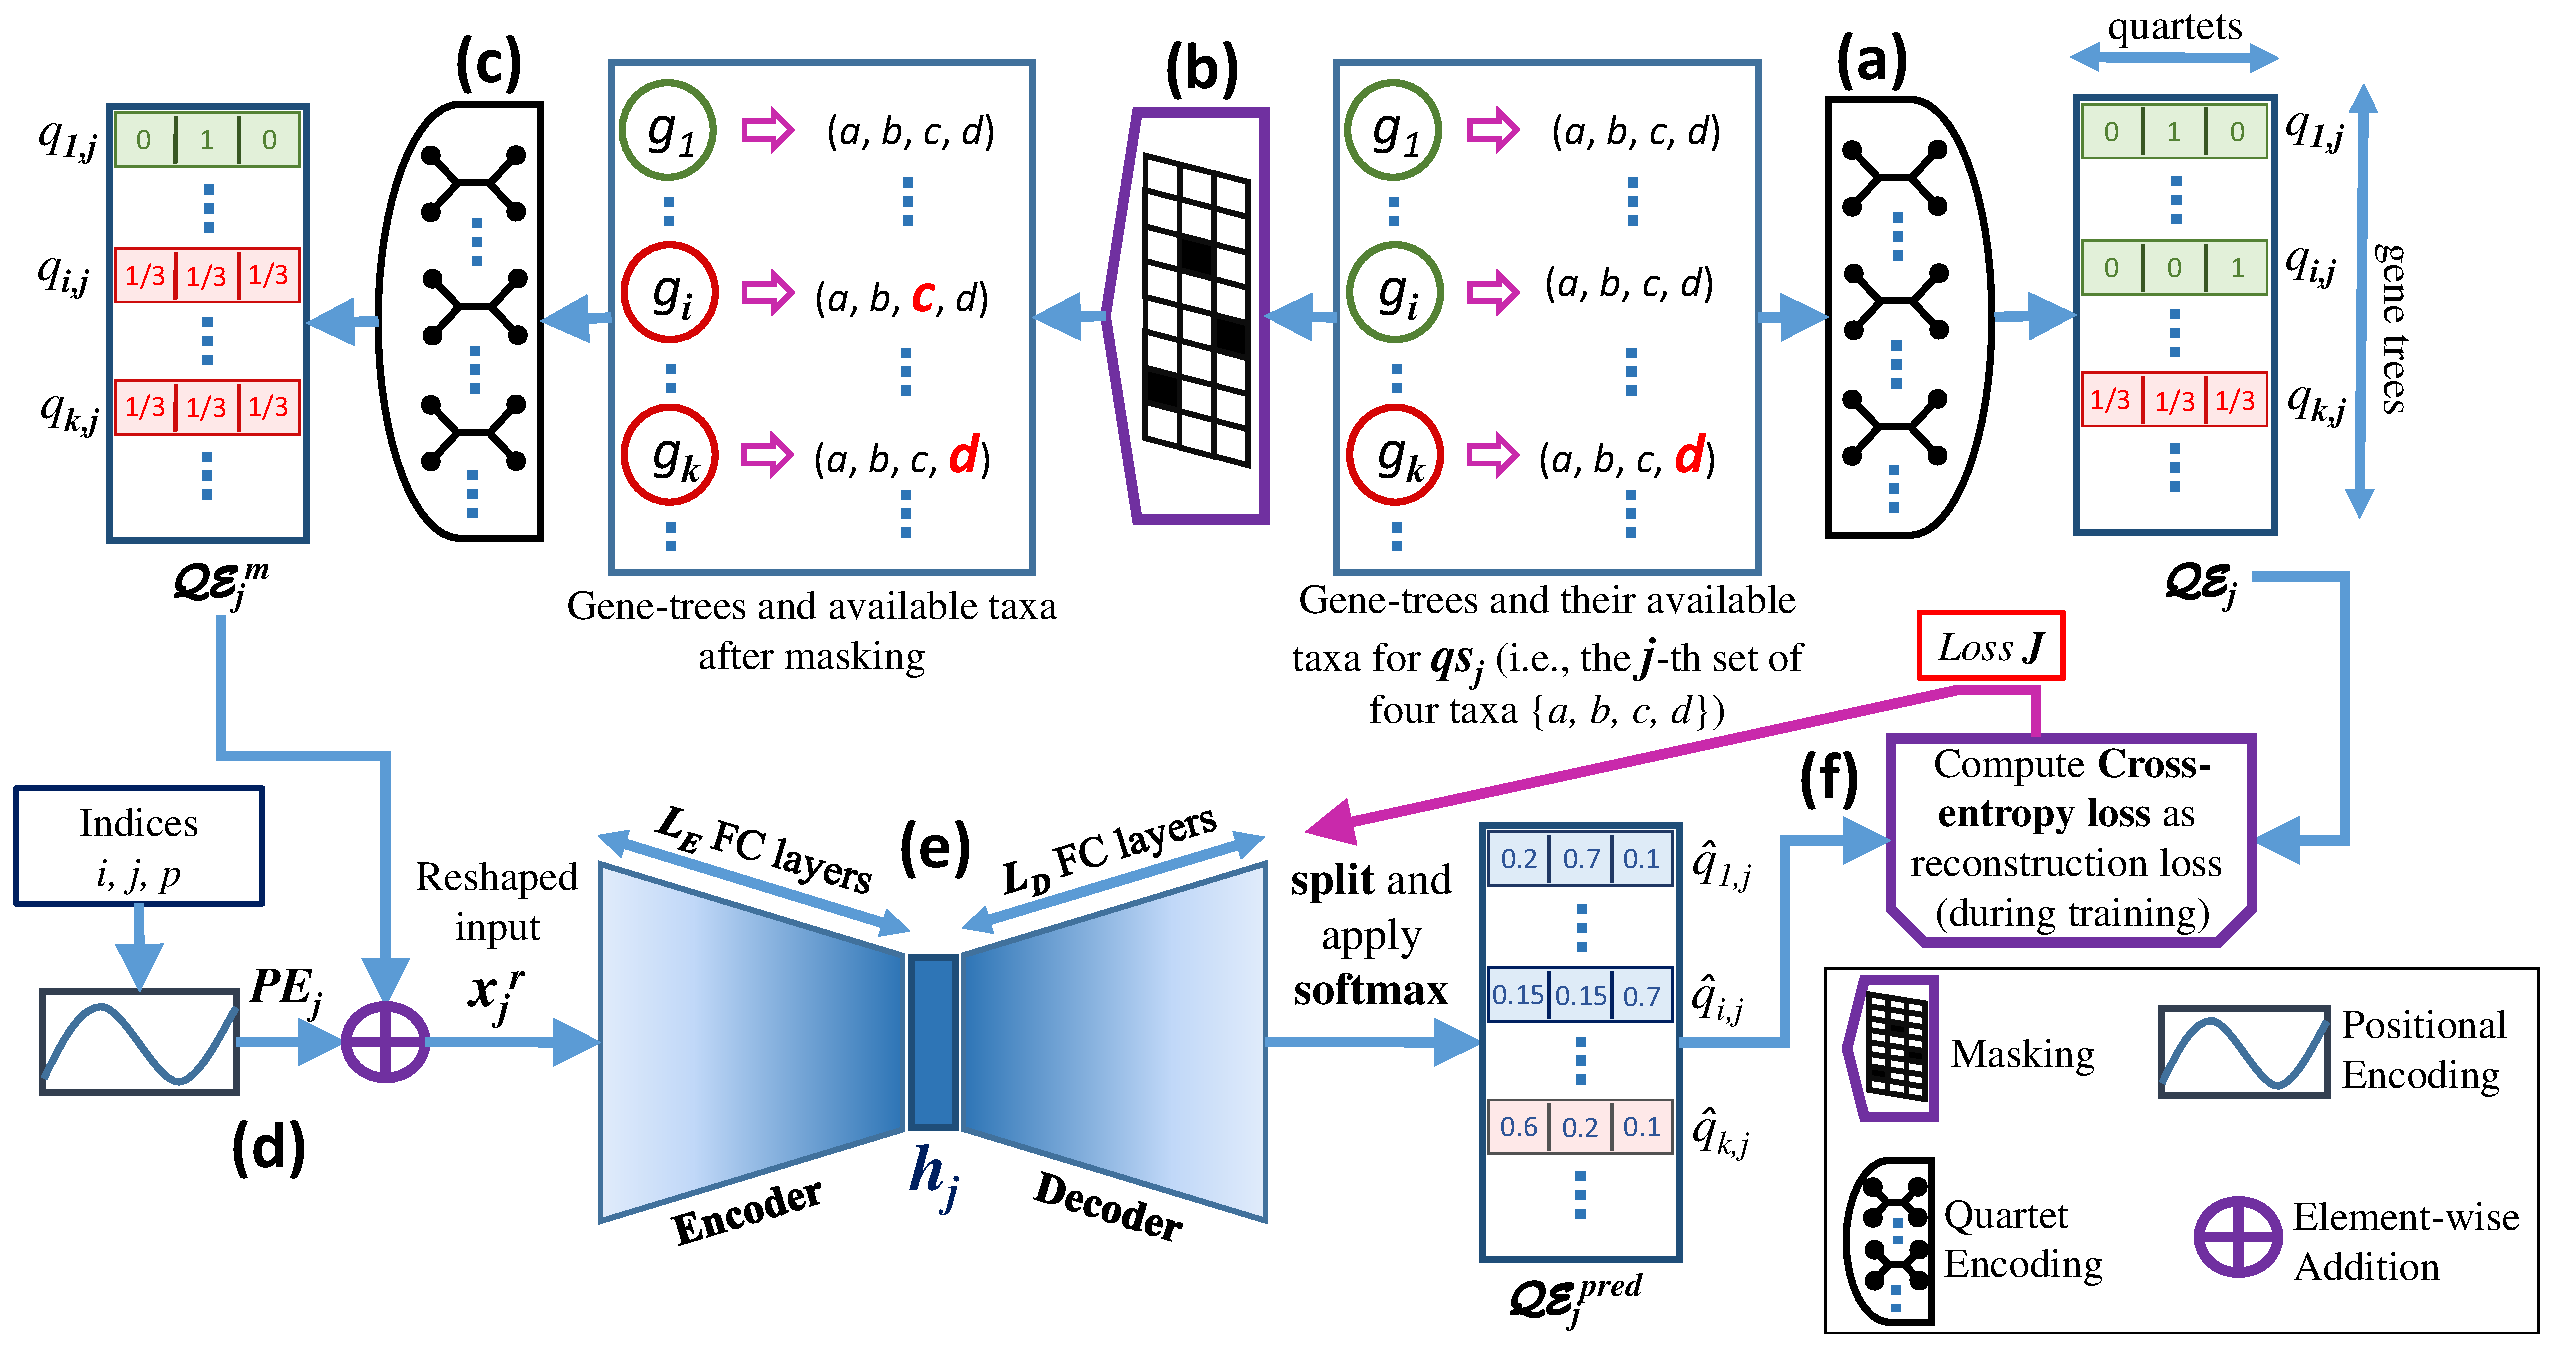
\includegraphics[width=1.\textwidth]{figures/imputation_pipeline.pdf}
    % \includegraphics[width=\textwidth]{figures/interpretability_protein_3ourA/AA90_neighbors.pdf}
    \caption{
    \textbf{Overall pipeline of QT-GILD.} (a) Generation of \textit{Quartet Encoding} matrix $\mathcal{QE}_j$ for a set of four taxa, $qs_j$. (b) Masking (in this example, taxon $c$ was masked out from gene tree $g_i$). (c) Generation of \textit{masked quartet encoding} matrix $\mathcal{QE}^m_j$ from the output of masking. (d) Positional encoding $PE_j$ generation from indices $i, j, p$, which are the index of a gene tree, index of a set of four taxa, and index of a possible quartet topology, respectively. (e) The reshaped version of the element-wise summation of $\mathcal{QE}^m_j$ and $PE_j$ (i.e., $x^r_j$) is passed through the autoencoder and the output is split and normalized using softmax, generating $\mathcal{QE}^{pred}_j$. (f) Cross-entropy loss $J$ is computed between $\mathcal{QE}^{pred}_j$ and $\mathcal{QE}_j$ and optimized to update the parameters of the autoencoder (the backward arrow represents backpropagation through the network). 
    }
    \label{fig:imputation_pipeline}
    % \par
\end{figure}

%For a dataset of gene-trees with a total of N_c unique taxa, we represent the set of all of these taxa as T_c={ti|1<=i<=N_c} (where ti represents the i-th taxa in T_c). 
% Then we define the incomplete \SR{gene-trees} as follows-\\
%\SR{In this section, we will discuss how we encode the quartets in matrices which can be fed into the autoencoders. }

For a set $S$ of $n$ taxa in $\mathcal{G}$, there are $n \choose 4$ subsets of four different taxa. For a set $qs_j$ ($1\le j \le$ $n \choose 4$) of four taxa $a,b,c,d \in S$, there are three possible quartets: $ab|cd$, $ac|bd$, and $ad|bc$. For a set of four taxa $qs_j$ and a gene tree $g_i \in \mathcal{G}$ ($1 \le i \le k$), we define a \textit{quartet vector} $q_{i,j}$ which represents a probability distribution of the presence of the three possible quartets in $g_i$. If $qs_j \cap \mathcal{MT}_i = \phi$ (meaning that $a,b,c,d$ are present in $g_i$), and without loss of generality $ab|cd \in \mathcal{Q}_i$, then $q_{i,j} = (1,0,0)$, where $1$ represents the presence of $ab|cd$ and the other two $0$s represent the absence of $ac|bd$ and $ad|bc$ in $\mathcal{Q}_i$. When $qs_j \cap \mathcal{MT}_i \ne \phi$ (i.e., there is no quartet on $qs_j$ in $\mathcal{Q}_i$), we set $q_{i,j} = (\frac{1}{3},\frac{1}{3},\frac{1}{3})$, representing a missing quartet which needs to be imputed and equal probabilities of the three possible quartets topologies for imputation. Next, for a particular set $qs_j$ of four taxa, we define a $k \times 3$ \textit{quartet encoding} matrix $\mathcal{QE}_j \in \mathbb{R}^{k \times 3}$ where the $i$-th row represents the quartet vector $q_{i,j}$. See Fig.~\ref{fig:quartet_vector} in Appendix \ref{app:quartet_encoding} for an example.


\subsubsection{Masking for self-supervision}
\label{sec:masking}
%%% Dr. Yann LeCun's fb post on self-supervised learning's definition: https://www.facebook.com/722677142/posts/10155934004262143/

We particularly aimed for developing an unsupervised autoencoder based model, but in order to increase the learning capability of our model in a supervised manner, we make it a \textit{self-supervised} model where a portion of the input is used as a supervisory signal to the autoencoder fed with the remaining portion of the input. In this context, we leverage a technique called ``masking'', which has been used in several state-of-the-art language modeling approaches, where we mask out a certain percentage of non-missing quartets in a quartet encoding matrix $\mathcal{QE}_j$, and ask the autoencoder to predict the masked quartets. 

We mask out randomly selected $\lambda|S|$ ($0 \le \lambda < 1$) non-missing quartets by replacing the one-hot encoded quartet vectors corresponding to the randomly selected non-missing quartets by $(\frac{1}{3},\frac{1}{3},\frac{1}{3})$.  Thus, we create a masked quartet encoding matrix $\mathcal{QE}_j^m$ from the original matrix $\mathcal{QE}_j$. During the training, the autoencoder takes $\mathcal{QE}_j^m$ as input and tries to predict the masked quartet vectors. The corresponding cross entroypy loss $J$ as the reconstruction loss (error) of predicting the masked entries with respect to the original quartet encoding matrix $\mathcal{QE}_j$ is computed and used as a feedback. Thus, the autoencoder is trained iteratively by backpropagating the loss $J$ within a feedback-loop, transforming a fully unsupervised approach into a self-supervised autoencoder and thereby helping the model to effectively learn the quartet distribution. %(\addb{see Fig. XYZ}). %making it a self-supervised autoencoder model (see Fig. XYZ).  (sazan: when do we stop training? when the loss is below a certain threshold?)


\begin{comment}

In order to convert this \textit{fully unsupervised} approach into a \textit{self-supervised} one, we use masking as shown in Figure \ref{fig:imputation_pipeline}(b) and Figure \ref{fig:imputation_pipeline}(c). This approach is widely used by several state-of-the-art language modeling approaches~\citep{BERT,Roberta,DistilBERT}. For this we mask out randomly selected $\frac{K * N^t_k}{100}$ taxa (Figure \ref{fig:imputation_pipeline}(b)) from the known taxa-set $T^t_k$ (where, $K$ is a hyperparameter representing the percentage of taxa-removal during masking) 
% $K$ (a hyperparameter) percentage of all taxa from the known taxa-set $T^t_k$ (masking) 
%which generates T_{masked} 
and from the remaining known taxa we generate another quartet-encoding matrix $Q^{m}_i \in \mathbb{R}^{N_G \times 3}~(\forall S_i \in S)$ using the aforementioned procedure (in Section \ref{sec:quartet_encoding}) as shown in Figure \ref{fig:imputation_pipeline}(c). This way, we end up with a set of indices ${Mask}_i = \{j ~|~ Q^m_i(j) = (\frac{1}{3},\frac{1}{3},\frac{1}{3}) ~\mbox{and}~ Q_i(j) \neq (\frac{1}{3},\frac{1}{3},\frac{1}{3})\}$ (here, $Q^m_i(j)$ and $Q_i(j)$ are the $j$-th element of $Q^m_i$ and $Q_i$ respectly). 
While training, the autoencoder will try to \textit{predict} the quartet-vectors $\{q_j \in Q_i ~|~ j \in {Mask}_i\}$ using $Q^{m}_i$ as input and their corresponding loss can be computed in a \textit{fully supervised fashion} considering $Q_i$ as the output. For the rest of the quartet-vectors $\{q_j \in Q_i ~|~ j \notin {Mask}_i ~\mbox{and}~ q_j \neq (\frac{1}{3},\frac{1}{3},\frac{1}{3})\}$ the autoencoder will try to \textit{reconstruct} those vectors from the input $Q^m_i(j)$. 
% Now, our autoencoder can predict those missing quartets based on the information of the existing quartets in $Q^{m}_i$ and train in a fully supervised manner for those quartets, while for the rest of the quartets 
% This provides us with an \SR{opportunity} to apply supervision for those specific four-taxa-sets, while the rest of the data are still used for pure autoencoding. \SR{To self: the next line sounds redundant. rephrase or delete this line:} 
\SR{Such a setup lets us transform a fully unsupervised approach into a self-supervised one, helping the model to learn better.}

\end{comment}

\subsubsection{Positional encoding}
\label{sec:positional_encoding}

Masked quartet encoding matrices $\mathcal{QE}_j^m$, $1 \le j \le$ $n\choose4$ defined on $n\choose4$ subsets of four taxa $qs_1, qs_2, \ldots, qs_{n\choose4}$ encode the information regarding three possible quartets on different four taxa set across all the gene trees in $\mathcal{G}$. However, $\mathcal{QE}_j^m$ does not encode any information about $qs_j$, making it impossible for the autoencoder to identify which set of four taxa is represented by a particular $\mathcal{QE}_j^m$.
%For each of the $n\choose4$ subsets of four taxa: $qs_1, qs_2, \ldots, qs_{n\choose4}$, we create a masked quartet encoding matrix $\mathcal{QE}_i^m$, $1 \le i \le$ $n\choose4$. $\mathcal{QE}_i^m$ encodes the information regarding three possible quartets on $qs_i$ across all the gene trees in $\mathcal{G}$, but it does not encode any information about $qs_i$, making it impossible for the autoencoder to identify which set of four taxa is represented by a particular $\mathcal{QE}_i^m$. 
%(\addb{Sazan: why is it necessary? we use the encodability matrix separately and imputes them separately. so why do we need to distinguish them. We need to write the motivation.}) 
In order to inject some information about different sets of four taxa, we incorporate an extra non-learnable signal, \textit{positional-encoding} (PE)~\cite{Transformer}. PE was originally proposed for NLP by Vaswani \textit{et al.}~\cite{Transformer} and is widely used to encode positional information of the tokens in sequence data. Recently, it has also been successfully applied to computational biology~\cite{SAINT}. For the $j$-th four-taxa-set $qs_j$, we generate a $k \times 3$ positional-encoding matrix $PE_j \in \mathbb{R}^{k \times 3}$ according to Equation \ref{eq:pos_enc}.

\vspace{-5pt}
\begin{equation}
\label{eq:pos_enc}
    PE_j(i, p) = \begin{cases} 
        sin{(j/{10000^{i/k}})}, & \mbox{if i is even} \\ 
        cos{(j/{10000^{(i-1)/k}})} & \mbox{if i is odd}   
    \end{cases} 
\end{equation}


Here, $PE_j(i, p)$ represents the positional-encoding of the $p$-th possible quartet ($1 \le p \le 3$) on $qs_j$ for the $i$-th gene tree $g_i \in \mathcal{G}$ and $|\mathcal{G}| = k$. Note that this function is constant with respect to $p$ 
% because the values are repeated $\forall q \in \{1,2,3\}$ 
% (considering zero-indexing) 
so that we get the same positional-encoding for three possible quartets on $qs_j$ for a particular gene tree $g_i$. 
The output of positional encoding $PE_j$
is element-wise added with $\mathcal{QE}_j^m$, resulting in new representations $X_j \in \mathbb{R}^{k \times 3}$
which contain not only the information about three possible quartets across all the gene trees, but also the information about different sets of four-taxa $qs_j$, $1 \le j \le $$n\choose 4$ (see Eqn. \ref{eqn:pos-and-qe} and Fig. \ref{fig:imputation_pipeline} (d)).

\vspace{-5pt}
\begin{equation}
\label{eqn:pos-and-qe}
X_j = PE_j + \mathcal{QE}_j^m
\end{equation}

%After this, $Q^{m}_i$ and $PEnc_i$ are added element-wise to produce the input of the autoencoder. The aforementioned process is decipted for a dummy dataset in Figure \ref{fig:imputation_pipeline} (d).




\begin{comment}

The $i$-th masked quartet-encoding matrix $Q^{m}_i \in \mathbb{R}^{N_G \times 3}$ contains the information about the quartets formed by any four-taxa-set $S_i \in S$ for all the gene-trees, but it does not encode any information about $S_i$ itself. As a results, for the autoencoder, all these matrices $\{Q^{m}_i~|~i \in [1, N_S]\}$ are equivalent -- making it is impossible for the autoencoder to learn to identify which four-taxa-set is represented by $Q^{m}_i$. 
%but this does not contain any information about which four-taxa-set is represented by $Q_{m}$. 
%As a result, using Q directly as input to our autoencoder does not provide 
In order to encode the information about the difference between all the possible four-taxa-sets $S$, we incorporate an extra non-learnable signal, \textit{Positional-Encoding}~\citep{Transformer}. Positional-Encoding has been proposed by Vaswani \textit{et al.}~\citep{Transformer} and is widely used to encode the positional information of the tokens in sequence data. Recently its usage has also been visible for research problems in computational biology~\citep{SAINT}. 
%To incorporate this, 
% we first stack up the orientation-encoding matrix for all the four-taxa-sets S_i SUBSET T_c (total N_c(C)4 four-taxa-sets). This generates a three-dimensional tensor, namely the stacked orientation encoding Q_{stacked} IN R^{N_c(C)4 x N_G x 3}. 
For the $i$-th four-taxa-set $S_i \in S$, we generate a positional-encoding matrix $PEnc_i \in \mathbb{R}^{N_G \times 3}$ according to Equation \ref{eq:pos_enc}. %$PEnc$ \SR{contains an extra(?) non-learnable signal that} helps the autoencoder to differentiate between not only the gene-trees but also the four-taxa-sets.

% EQ… PEnc_{(s, 2t, o)}=…

\begin{equation}
\label{eq:pos_enc}
    PEnc_i(t, p) = \begin{cases} 
        sin{(i/{10000^{t/d_{feature}}})}, & \mbox{if ``t is even''} \\ 
        cos{(i/{10000^{(t-1)/d_{feature}}})}, & \mbox{\SR{else if ``t is odd''}}   
    \end{cases} 
\end{equation}

% \begin{equation}
% \label{eq:pos_enc}
%     PEnc_i(t, q) = \begin{cases} 
%         sin{(\frac{i}{{10000^{\frac{t}{d_{feature}}}}})}, & \mbox{if ``t is even''} \\ 
%         cos{(\frac{i}{{10000^{\frac{t-1}{d_{feature}}}}})}, & \mbox{else if ``t is odd''}   
%     \end{cases} 
% \end{equation}

% \SR{Define the set of gene-tree G\\}
Here, $PEnc_i(t, p)$ represents the positional-encoding of the $p$-th possible quartet formed by the four-taxa-set $S_i$ for the $t$-th gene tree $g_t \in G$. 
% \SR{ to self : change 2t (even) and 2t+1 (odd) to a single variable t, in a single equation}. 
Here, we can see that the function is constant with respect to the variable $p$ 
% because the values are repeated $\forall q \in \{1,2,3\}$ 
% (considering zero-indexing) 
so that we get the same positional-encoding for all possible quartets formed by $S_i$ for $g_t$. After this, $Q^{m}_i$ and $PEnc_i$ are added element-wise to produce the input of the autoencoder. The aforementioned process is decipted for a dummy dataset in Figure \ref{fig:imputation_pipeline} (d).
% which generates $X \in \mathbb{R}^{N_G \times 3}$, the input of our deep autoencoder. 

% \SR{??? --> $^{N_c}C_{4}$ or $\binom{N_c}{4}$}

\end{comment}

\subsubsection{Deep autoencoder}
\label{sec:autoencoder}

Autoencoder (AE)~\cite{goodfellow2016deep} is a type of artificial neural network that learns to copy its input to its output. The deep autoencoder architecture consists of two modules -- encoder and decoder -- stacked one after the other and built using fully-connected layers (Figure \ref{fig:imputation_pipeline} (e)). 
%The deep autoencoder architecture consists of two modules -- encoder and decoder -- stacked one after the other and built using fully-connected layers\SR{[cite]} (Figure \ref{fig:imputation_pipeline} (e)). 
%For all $i \in [1, N_S]$, 
The output $X_j$ of the element-wise summation of $\mathcal{QE}^{m}_j$ and $PE_j$ (as discussed in Section \ref{sec:positional_encoding}) is reshaped into a vector $x^r_j \in \mathbb{R}^{k * 3}$, which is used as the input of the encoder module. By using subsequent $L_E$ fully-connected layers, the dimension of $x^r_j$ is reduced and a condensed latent representation $h_j$ is generated, which is subsequently used as the input of the decoder module. In the decoder, the dimension of $h_j$ is expanded by $L_D$ fully-connected layers (here, $L_E$ and $L_D$ are two hyperparameters). 
The output of the $L_D$-th layer is divided into $k$ equal segments of length $3$ %in an exact order \addb{what is exact order?} 
and softmax normalization is applied on each of them. Here, softmax on the $i$-th segment generates the predicted quartet-vector $\hat{q}_{i,j}$, which is the estimated probability distribution over the possible quartets on $qs_j$ for the gene-tree $g_i$. Thus, $\forall g_i \in \mathcal{G}$, we get $\mathcal{QE}^{pred}_j = [\hat{q}_{1,j}, \hat{q}_{2,j}, \dots, \hat{q}_{k,j}]$, which is the predicted quartet-encoding matrix corresponding to $qs_j$. 
%For the whole stacked orientation-encoding tensor $Q_{stacked} \in \mathbb{R}^{\binom{N_c}{4} \times N_G \times 3}$ (discussed in Section ??), the autoencoder generates the output tensor $Q_{pred}  \in \mathbb{R}^{\binom{N_c}{4} \times N_G \times 3}$ which contains not only the information about the quartets that were present in the dataset, but also the \textit{missing quartets} (defined in Section ??). Here, $K_E$ and $K_D$ are two hyperparameters of the autoencoder. In our final architecture $K_E=K_D=\SR{Check the code}$. 


% \subsection{Overall Pipeline of \methodname OLD}
% In this section, we discuss the overall pipeline of our method \methodname applied on a dataset of incomplete gene-trees.
% As shown in Figure ?? and described in Section ??, in the first step, a stacked orientation-encoding $Q_{stacked}$ is generated from the gene-trees. Then a masking is applied on it to generate a separate tensor $Q_{masked}$ (shown in Figure ?? and described in Section ??). $Q_{masked}$ is added (element-wise) with positional-encoding matrix $PEnc$ (shown in Figure ?? and described in Section ??) and passed through the deep autoencoder that generates the \SR{predicted stacked orientation-encoding} $Q_{pred}$. $Q_{pred}$ is then compared with $Q_{stacked}$ to calculate the cross-entropy loss\SR{[cite]} as the reconstruction loss\SR{[cite]}. The whole model is then trained with backpropagation\SR{[cite]} 
% % this loss through the whole model 
% until convergence.

% % EQ..

% % As discussed in Section ??, the aforementioned process lets us train our model in a self-supervised manner. We use the converged model as the final predictor and its output $Q_{pred}$ is used to fill up the missing-quartets (defined in Section ??) in $Q_{stacked}$ and generate the final imputed tensor Q_{imputed}. This process is shown in Figure ??. 
% After this, for each possible four-taxa-set, we pick the orientation with the highest probability from three possible orientations as the \textit{predicted quartet} using the probability distributions that are available in $Q_{pred}$. Let, the set of such \textit{predicted quartets} for all four-taxa-set in a specific gene-tree be $S_{p}$  and the set of the known quartets in that tree be $S_{k}$, where $|S_{p}|=\binom{N_c}{4}$ and $|S_{k}|=\binom{N_k}{4}$. Then we can compute the set of only predicted (but not previously known) quartets, $\hat{S}_{p}$, using set operation as shown in Equation \ref{eq:s_hat_P}.

% \begin{equation}
% \label{eq:s_hat_P}
% \hat{S}_{p} = S_p - S_k
% \end{equation}

% Using $\hat{S}_{p}$ and $S_k$ we can generate the final set of imputed quartets $S_\mathcal{I}$ following Equation \ref{eq:s_i}. %[Sazan: ekhane S_I er I ta mathcal kore dao].

% \begin{equation}
% \label{eq:s_i}
% S_\mathcal{I} = \hat{S}_{p} \cup S_k
% \end{equation}

% For all the gene trees in our dataset, we apply the aforementioned process and this generates a list of sets of imputed quartets $L_\mathcal{I}$. Similarly, we generate a list of sets of known quartets $L_k$. $L_\mathcal{I}$ and $L_k$ are used to estimate the species trees $ST_I$ and $ST_k$ respectively, using the widely used method wQMC \SR{[cite]}. $ST_I$ and $ST_k$ are compared with the true species tree $ST_{true}$ to calculate the error rates that depict the performance of our method, i.e, how well our method could improve the species tree estimation by using the discussed imputation technique.

% %We use these predicted quartets to fill up the missing quartets (discussed in Section ??) in Q_{stacked} and this generates the set of quartets for all the ...
% %This provides us with a set of 



\subsubsection{Overall pipeline of QT-GILD}
\label{sec:overall_pipeline}

\begin{comment}
\begin{figure}[htbp]
    \centering
    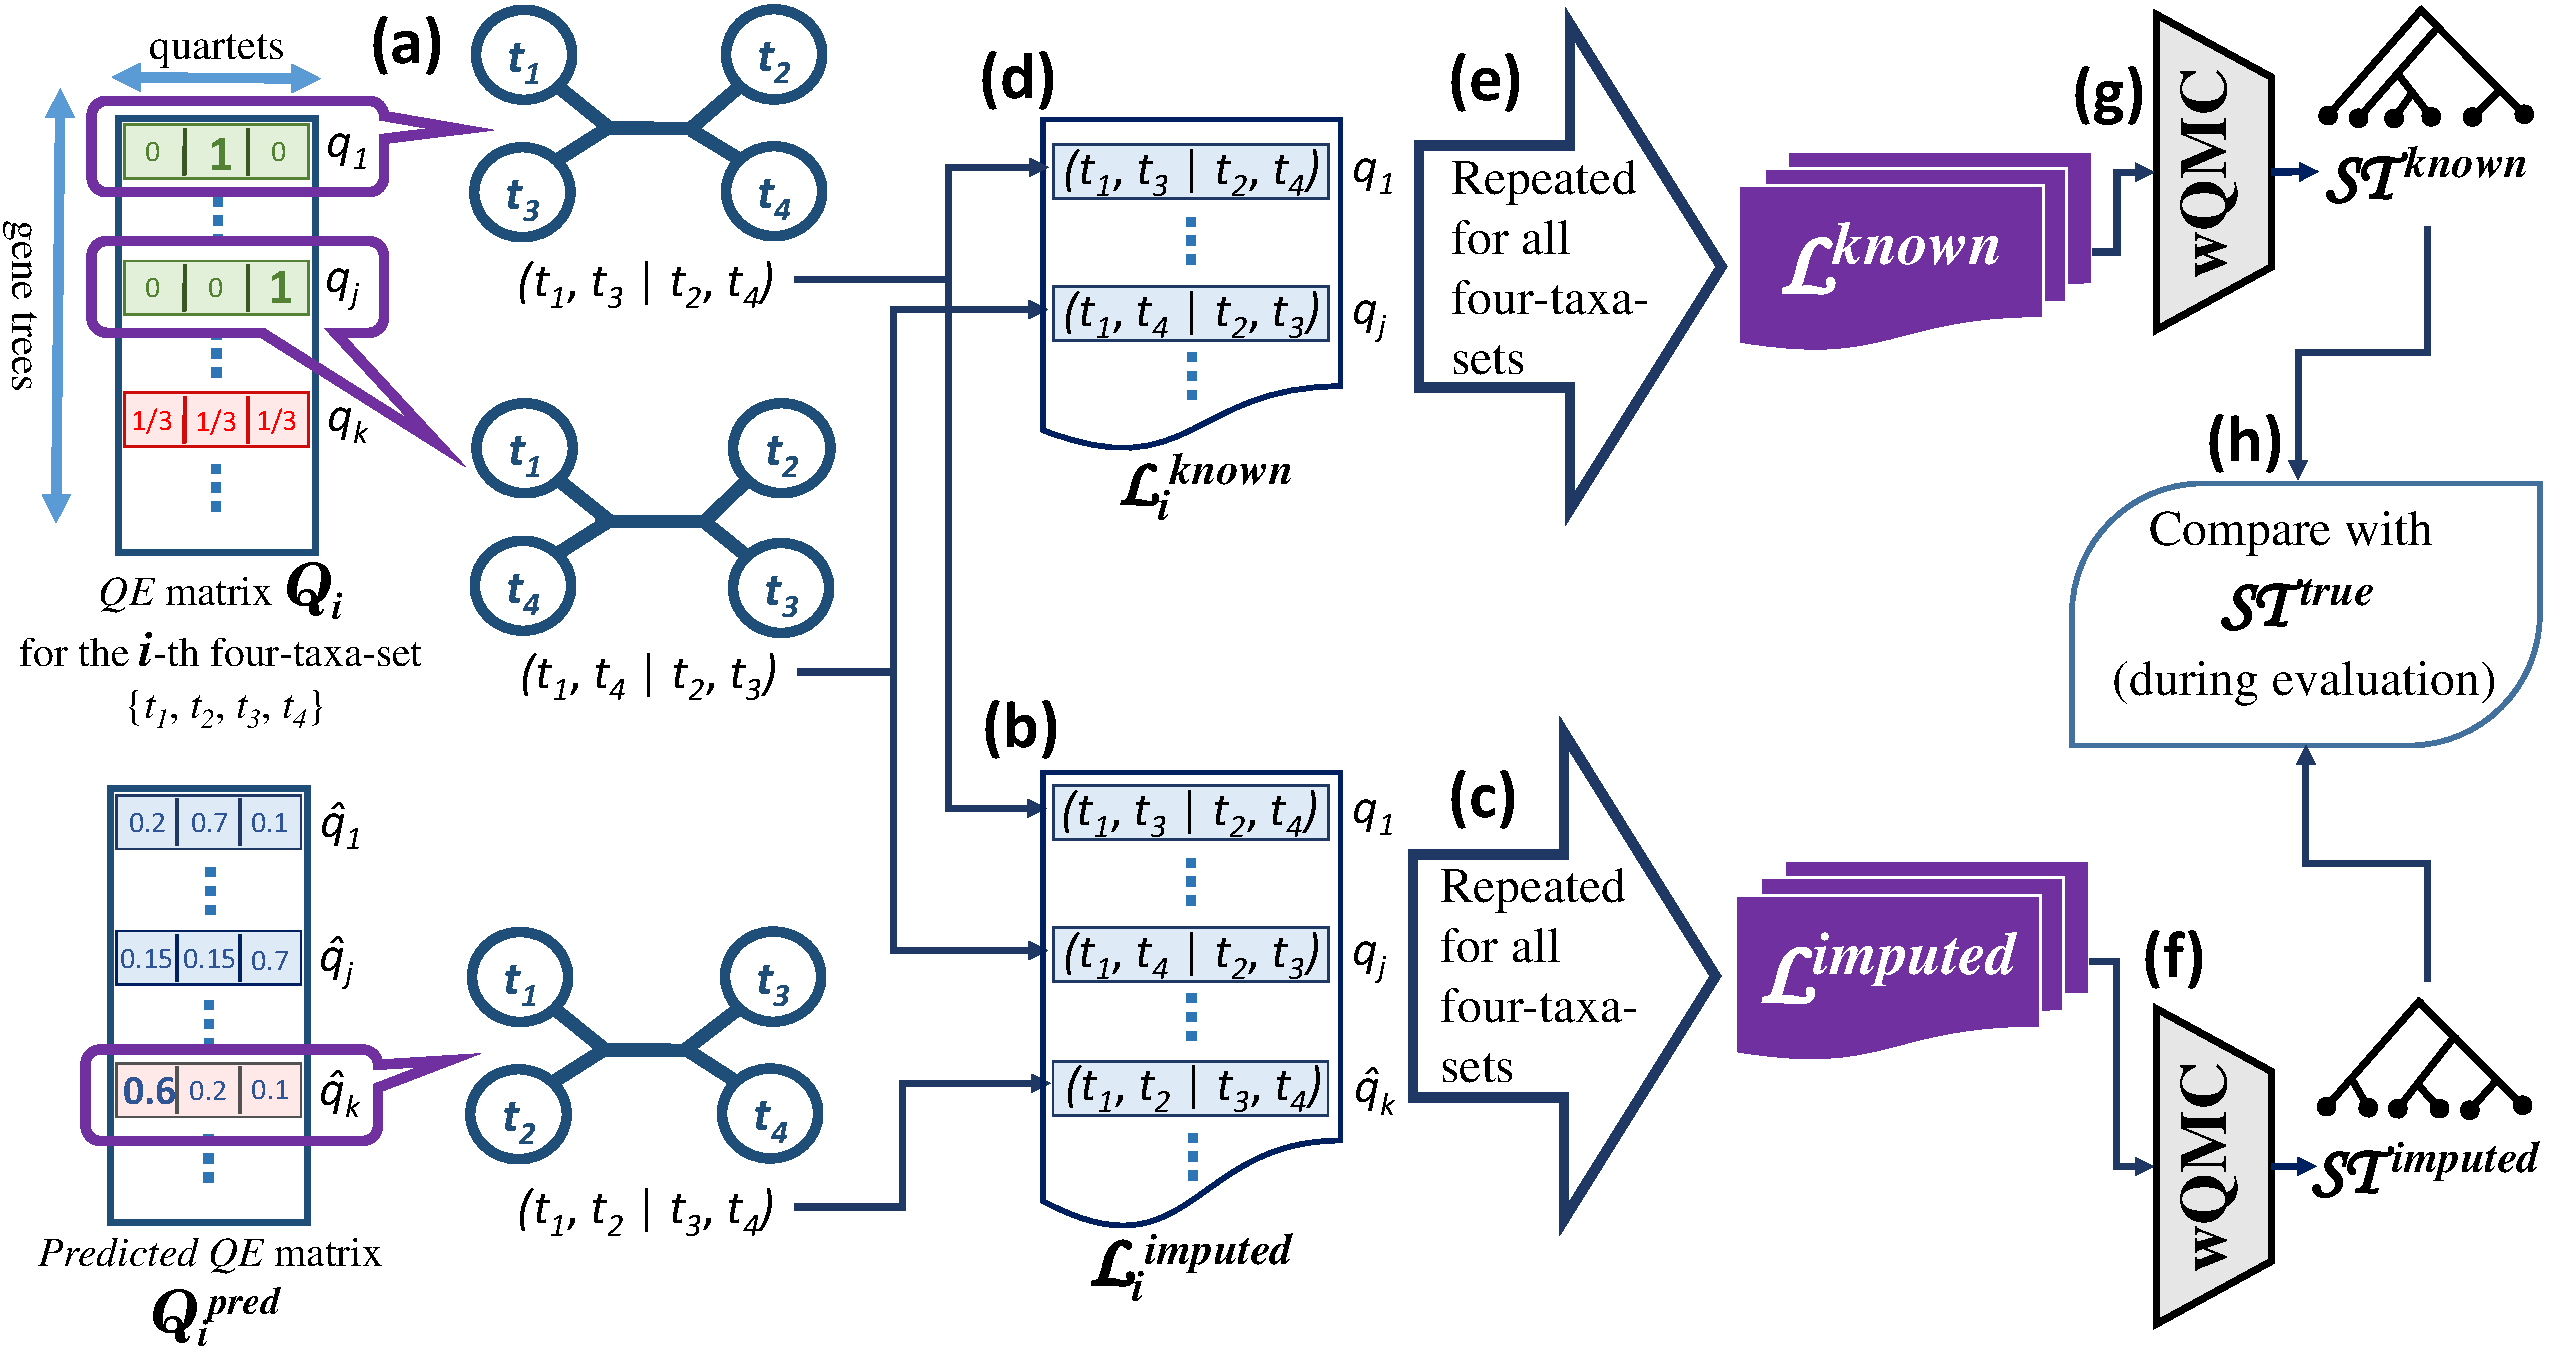
\includegraphics[width=1.\textwidth]{figures/ST_estimation.pdf}
    % \includegraphics[width=\textwidth]{figures/interpretability_protein_3ourA/AA90_neighbors.pdf}
    \caption{
    \textbf{}
    }
    \label{fig:ST_estimation}
    % \par
\end{figure}
\end{comment}

Figure~\ref{fig:imputation_pipeline} shows the overall end-to-end pipeline of QT-GILD comprising the individual components described in Sections 2.2-2.5. For each set of four taxa $qs_j$, we first create a quartet encoding matrix $\mathcal{QE}_j$, which is subsequently masked to produce $\mathcal{QE}^m_j$. Next, these masked encoding matrices are added to positional encoding matrices and reshaped to generate the input $x_i^r$ of the autoencoder. The autoencoder network produces the predicted quartet-encoding matrix $\mathcal{QE}^{pred}_j$. During the training phase, considering $\mathcal{QE}^{pred}_j$ as the prediction and $\mathcal{QE}_j$ as the ground truth, we compute the cross-entropy loss $J$ as the reconstruction loss for the non-missing quartets, i.e., for the quartet-vectors $\{q_{i,j} ~|~ q_{i,j} \in \mathcal{QE}_j ~\mbox{and}~ q_{i,j} \neq (\frac{1}{3},\frac{1}{3},\frac{1}{3})\}$. The autoencoder is trained by backpropagating  this loss in a self-supervised fashion (see Fig.~\ref{fig:imputation_pipeline}(f) and Section \ref{sec:masking}). This training with backpropagation is run for a predefined number of epochs. Finally, it is run once without the loss function to produce the final encoding matrix $\mathcal{QE}^{pred}_j$. %Next, we generate the set of imputed quartets  $\mathcal{L}^{imputed}_i(k)$ -- representing the quartets in the $k$-the gene-tree -- as computed according to Equation~\ref{eq:q_imputed}. This imputed set of quartets is subsequently used by quartet amalgamation techniques, such as wQFM and wQMC.
Next, we generate the set of imputed quartets  $\mathcal{L}^{imputed}_i$ -- representing the quartets in the $i$-the gene-tree $g_i$ -- as computed according to Equation~\ref{eq:q_imputed}. This imputed set of quartets is subsequently used by quartet amalgamation techniques, such as wQFM and wQMC.

\vspace{-5pt}
\begin{equation}
\label{eq:q_imputed}
    \mathcal{L}^{imputed}_i(k) = \begin{cases} 
        \mbox{quartet corresponding to}~Argmax(\mathcal{Q}_i(j)), & \mbox{if}~ \mathcal{Q}_i(j) \neq (\frac{1}{3},\frac{1}{3},\frac{1}{3}) \\ 
        \mbox{quartet corresponding to}~Argmax(\mathcal{Q}^{pred}_i(j)), & \mbox{otherwise}   
    \end{cases} 
\end{equation}


\begin{comment}
% \subsubsection{Imputation of Gene-trees Dataset}

As depicted in Figure \ref{fig:imputation_pipeline}(a), firstly the available taxa of the $i$-th four-taxa-set $S_i \in S$ are recognized from all the incomplete gene-trees of a certain dataset and our Quartet-Encoding Module, according to the process discussed in Section \ref{sec:quartet_encoding}, encodes them into a quartet-encoding matrix $Q_i$. On the other hand, according to Section \ref{sec:masking}, masking is applied on the dataset (Figure \ref{fig:imputation_pipeline}(b)) and its output is also passed through Quartet-Encoding Module (Figure \ref{fig:imputation_pipeline}(c)) which generated the masked quartet-encoding matrix $Q^m_i$. After this, the index of $S_i$ in the list S, along with the indices of the quartet-vectors $q_j \in Q^m_i$, is passed through the Positional-Encoding Module; this generates the positional encoding matrix which is added element-wise with $Q^m_i$ (as discussed in Section \ref{sec:positional_encoding}) and reshaped to generate the input of the autoencoder $x^r_i$ (depicted in Figure \ref{fig:imputation_pipeline}(d)). As we can see in Figure \ref{fig:imputation_pipeline}(e), from the input $x^r_i$, the autencoder generates the predicted quartet-encoding matrix $Q^{pred}_i$ (discussed in Section \ref{sec:autoencoder}). Considering $Q^{pred}_i$ as the prediction and $Q_i$ as the label, we compute the cross-entropy loss $J$ as the reconstruction loss during training (Figure \ref{fig:imputation_pipeline}(f)) for only the quartet-vectors $\{q_j ~|~ q_j \in Q_i ~\mbox{and}~ q_j \neq (\frac{1}{3},\frac{1}{3},\frac{1}{3})\}$ (i.e., only for the initially known quartets) and the autoencoder is trained by backpropagation of this loss in a self-supervised fashion (discussed in Section \ref{sec:masking}). 

The aforementioned process is repeatedly run during training for all $S_i \in S$ until convergence. After the model converges, this process is run one last time except for the loss calculation and this generates the final $Q^{pred}_i$ and $Q_i$ (for $S_i \in S$); these are used to compute the final imputed list of quartets $\mathcal{L}^{imputed}_i$ (Figure \ref{fig:ST_estimation}(b)), where the $k$-th element $\mathcal{L}^{imputed}_i(k)$ -- representing the estimated or true quartet in the $k$-the gene-tree -- is computed according to Equation \ref{eq:q_imputed} (shown in Figure \ref{fig:ST_estimation}(a)). 
\begin{equation}
\label{eq:q_imputed}
    \mathcal{L}^{imputed}_i(k) = \begin{cases} 
        \mbox{quartet corresponding to}~Argmax(Q_i(j)), & \mbox{if}~ Q_i(j) \neq (\frac{1}{3},\frac{1}{3},\frac{1}{3}) \\ 
        \mbox{quartet corresponding to}~Argmax(Q^{pred}_i(j)), & \mbox{otherwise}   
    \end{cases} 
\end{equation}
% Latex font "\matcal" == powerpoint font "monotype corsiva"
Here, $Q^{pred}_i(j)$ and $Q_i(j)$ are the $j$-th element of $Q^{pred}_i$ and $Q_i$ respectively. Equation \ref{eq:q_imputed} shows that $\mathcal{L}_i(k)$ is formed by taking the initially known quartets from $Q_i$ (by doing an $Argmax(.)$ operation) and the rest (i.e., initially missing) from $Q^{pred}_i$ for the $i$-the four-taxa-set. Here $Argmax(.)$ operation represents a function that returns the index of the maximum value in a list; in our case this index represents a possible quartet formed by the four-taxa-set $S_i$. For all $S_i \in S$, we get $\mathcal{L}^{imputed} = [\mathcal{L}^{imputed}_i(1), \mathcal{L}^{imputed}_i(2), \dots, \mathcal{L}^{imputed}_i(N_G)]$ (Figure \ref{fig:ST_estimation}(c)). Similarly, we generate a list for only known quartets $\mathcal{L}^{known}$, but here we do not take any predicted quartets into consideration (Figure \ref{fig:ST_estimation}(d) and Figure \ref{fig:ST_estimation}(e)). Then $\mathcal{L}^{known}$ and $\mathcal{L}^{inputed}$ are used to estimate the species trees $\mathcal{ST}^{imputed}$ and $\mathcal{ST}^{known}$ respectively, using the widely used method wQMC~\citep{avni2015weighted} (Figure \ref{fig:ST_estimation}(f) and Figure \ref{fig:ST_estimation}(g)). During evaluation of our method, $\mathcal{ST}^{imputed}$ and $\mathcal{ST}^{known}$ are compared with the already available true species tree $\mathcal{ST}^{true}$ (Figure \ref{fig:ST_estimation}(h)) to calculate the error rates that depict the performance of our method, i.e, how well our method could improve the species tree estimation by using the discussed imputation technique.

\end{comment}

% The aforementioned process is repeatedly run during training for all $S_i \in S$ until convergence. After the model converges, this process is run one last time for all $S_i \in S$ except for the loss calculation and this generates the final $Q^{pred}_i$ and $Q_i$, which is used to compute the imputed quartet-encoding matrix $Q^{imputed}_i = [q_1, q_2, \dots, q_{N_G}]$, where the $k$-th element $q_k$ is computed according to Equation \ref{eq:q_imputed}. 
% \begin{equation}
% \label{eq:q_imputed}
%     q_k = \begin{cases} 
%         Q_i(j), & \mbox{if}~ Q_i(j) \neq (\frac{1}{3},\frac{1}{3},\frac{1}{3}) \\ 
%         Q^{pred}_i(j), & \mbox{otherwise}   
%     \end{cases} 
% \end{equation}
% Here, $Q^{pred}_i(j)$ and $Q_i(j)$ are the $j$-th element of $Q^{pred}_i$ and $Q_i$ respectly. Equation \ref{eq:q_imputed} shows that $Q^{imputed}_i$ is formed by taking the initially known quartets from $Q_i$ and the rest (i.e., initially missing) from $Q^{pred}_i$ for the $i$-the four-taxa-set.



% The aforementioned process is repeatedly run during training for all $S_i \in S$ until convergence. After the model converges, this process is run one last time for all $S_i \in S$ except for the loss calculation and this generates the final $Q^{pred}_i$ and $Q_i$, which is used to compute the imputed quartet-encoding matrix $Q^{imputed}_i = [q_1, q_2, \dots, q_{N_G}]$, where the $k$-th element $q_k \in \{q_j \in Q_i ~|~ Q_i(j) \neq (\frac{1}{3},\frac{1}{3},\frac{1}{3})\} \cup \{q_j \in Q^m_i ~|~  Q_i(j) = (\frac{1}{3},\frac{1}{3},\frac{1}{3})\} $. (here, $Q^m_i(j)$ and $Q_i(j)$ are the $j$-th element of $Q^m_i$ and $Q_i$ respectly). $Q^{imputed}_i$ is formed by taking the missing quartets from $Q^m_i$ and the available quartets from $Q_i$ for the $i$-the four-taxa-set.

% which is used to compute the imputed quartet-encoding matrix $Q^{imputed}_i = (q_k)_{1 \leq k \leq N_G}$, where $k \in \{j ~|~ Q_i(j) \neq (\frac{1}{3},\frac{1}{3},\frac{1}{3})\} \cup \{j ~|~ Q_i(j) \neq (\frac{1}{3},\frac{1}{3},\frac{1}{3}) ~\mbox{and}~ Q^m_i(j) \neq (\frac{1}{3},\frac{1}{3},\frac{1}{3})\} $. 

% which is used to compute the imputed quartet-encoding matrix $Q^{imputed}_i = (q_k)_{1 \leq k \leq N_G}$, where $k \in \{j ~|~ Q_i(j) \neq (\frac{1}{3},\frac{1}{3},\frac{1}{3})\} \cup \{j ~|~ Q_i(j) \neq (\frac{1}{3},\frac{1}{3},\frac{1}{3}) ~\mbox{and}~ Q^m_i(j) \neq (\frac{1}{3},\frac{1}{3},\frac{1}{3})\} $. 

% ${Mask}_i = \{j ~|~ Q^m_i(j) = (\frac{1}{3},\frac{1}{3},\frac{1}{3}) ~\mbox{and}~ Q_i(j) \neq (\frac{1}{3},\frac{1}{3},\frac{1}{3})\}$
